\section{Protocol}
\label{sec:protocol}

% ── Mark scheme: 15 marks ─────────────────────────────────────────────────────

\subsection{The Serial Link Carries Plain Text Lines of at Most 64 Bytes}

The STM32 communicates with the PC over \textbf{USART1} (pins PA9~TX, PA10~RX),
which is connected internally to the onboard ST-Link chip.
The ST-Link presents a \textbf{Virtual COM Port (VCP)} to the host operating system,
so no external USB-to-UART adapter is required.
The link parameters are 115\,200 baud, 8 data bits, no parity, 1 stop bit (8N1),
no hardware flow control.

A frame is a sequence of printable ASCII characters terminated by a newline
character (\texttt{\textbackslash n}, ASCII 0x0A).
Carriage return characters (\texttt{\textbackslash r}) are silently discarded,
so Windows-style \texttt{\textbackslash r\textbackslash n} line endings work
without any special handling.
No checksum or CRC is used; the link is short and the ST-Link USB transfer
provides its own error correction.
Table~\ref{tab:framing} summarises the framing rules.

\begin{table}[t]
\centering
\caption{Framing rules and the server's response to each condition.}
\label{tab:framing}
\footnotesize
\begin{tabular}{@{}L{2.8cm}L{5.2cm}@{}}
\toprule
Rule & Server behaviour \\
\midrule
Terminator          & \texttt{\textbackslash n} ends a frame; \texttt{\textbackslash r} is silently discarded \\
Maximum frame length & 64 bytes (excluding delimiter); excess bytes discarded, returns \texttt{NACK:BADCMD} upon \texttt{\textbackslash n} \\
Incomplete frame    & Discarded after 500\,ms timeout; returns \texttt{NACK:BADCMD} \\
Invalid character   & Accumulated until delimiter; rejected by command validator \\
Checksum            & None; short USB-VCP physical layer provides USB CRC \\
UART errors         & Hardware flags cleared in error ISR; receiver re-armed \\
\bottomrule
\end{tabular}
\end{table}

\subsection{The Board is Nine Characters, Left to Right, Top to Bottom}

The game board is encoded as a string of exactly nine characters.
Cell~0 is the top-left corner; cell~8 is the bottom-right corner, reading
left to right and top to bottom (row-major order).
An empty cell is a full stop (\texttt{.}); a cell owned by Player~X is the
letter \texttt{X}; a cell owned by Player~O is the letter \texttt{O}.

\textbf{Example.} After Player~X takes cell~0 and Player~O takes cell~4,
the board string is \texttt{X...O....}, which represents:

\begin{center}
\texttt{X | . | .} \\
\texttt{. | O | .} \\
\texttt{. | . | .}
\end{center}

\subsection{Commands Are Synchronous Uppercase ASCII Strings With Single-Line Replies}

Table~\ref{tab:commands} lists every command the server accepts.
All commands are case-sensitive uppercase ASCII.
A move command includes the player letter and the target cell index,
separated by colons: \texttt{MOVE:X:4} means ``Player~X requests cell~4.''
The server always responds with exactly one line before accepting the next command.

\begin{table}[t]
\centering
\caption{Complete command set. The serial link receives frames in any state, but command execution depends strictly on the current FSM state. Incompatible requests return \texttt{NACK:NOGAME} or \texttt{NACK:BADCMD}.}
\label{tab:commands}
\scriptsize
\begin{tabular}{@{}L{2.0cm}L{1.8cm}L{4.2cm}@{}}
\toprule
Request & Valid in & Success response \\
\midrule
\texttt{CONNECT}          & Any state        & \texttt{OK} (resets session to IDLE) \\
\texttt{NEW}              & IDLE, GAME\_OVER & \texttt{OK:BOARD:.........} \\
\texttt{MOVE:\textit{p}:\textit{i}} & IN\_PROGRESS & \texttt{OK:BOARD:\textit{grid}}, \texttt{WIN:\textit{p}}, or \texttt{DRAW} \\
\texttt{STATE}            & Any state        & \texttt{BOARD:\textit{grid}} \\
\texttt{RESIGN}           & IN\_PROGRESS     & \texttt{OK:GAMEOVER} \\
\texttt{DISCONNECT}       & Any state        & \texttt{OK} (resets session to IDLE) \\
\bottomrule
\end{tabular}
\end{table}

\subsection{Deterministic Error Codes Map Directly to Specific Rule Violations}

Table~\ref{tab:errors} lists every error response.
The order of checks inside \texttt{game\_process\_move()} matters because
a single bad command can fail more than one check.
The server applies them in a fixed sequence:
(1)~syntax and player token, (2)~game state, (3)~cell index range, (4)~turn order, and (5)~cell occupancy.
This ensures each rejected command yields an unambiguous, predictable error code.

\begin{table}[t]
\centering
\caption{Every error response and the exact condition that triggers it.}
\label{tab:errors}
\footnotesize
\begin{tabular}{@{}L{2.4cm}L{5.6cm}@{}}
\toprule
Response & Sent when \\
\midrule
\texttt{NACK:BADCMD}    & Unrecognised verb, frame $>64$ bytes, 500\,ms timeout, invalid player token (not \texttt{X} or \texttt{O}), or malformed syntax (e.g. missing colon or omitting player) \\
\texttt{NACK:NOGAME}    & \texttt{MOVE} or \texttt{RESIGN} received while in \texttt{IDLE} or \texttt{GAME\_OVER} \\
\texttt{NACK:RANGE}     & Move index is not a decimal digit or falls outside the valid range 0 to 8 \\
\texttt{NACK:NOTURN}    & Claiming player token does not match the active turn (\texttt{g\_current\_player}) \\
\texttt{NACK:OCCUPIED}  & The requested cell already contains \texttt{X} or \texttt{O} \\
\bottomrule
\end{tabular}
\end{table}

\subsection{Deliberate Protocol Design Choice: Explicit Player Tokens in Move Commands}

The reference protocol in the project brief~\cite{brief} specifies a move command of the form \texttt{MOVE:\textit{i}} (specifying the target cell index only).
Under that format, a server enforces alternating turns by assigning each incoming legal move to whichever player currently holds the active turn, advancing its internal turn counter automatically.
However, because \texttt{MOVE:\textit{i}} carries no player token, the server has no identity against which to validate the originator of the request; it cannot detect if a specific participant attempts to submit a move out of order.

As permitted by the project brief (which instructs teams to adapt the protocol and highlight departures from the reference), our implementation adopts \texttt{MOVE:\textit{p}:\textit{i}} as a deliberate design choice, where $p \in \{\texttt{X}, \texttt{O}\}$ denotes the claiming player token and $i \in \{0, \dots, 8\}$ denotes the target cell index.
This explicit player parameter allows the server to verify that the claimed identity matches the active player (\texttt{g\_current\_player}) before altering state, returning \texttt{NACK:NOTURN} if an out-of-order move is submitted (e.g., submitting \texttt{MOVE:X:1} immediately after \texttt{MOVE:X:0}).
If a client transmits the reference \texttt{MOVE:\textit{i}} format without the player prefix, the server's syntax validator rejects it deterministically with \texttt{NACK:BADCMD}.
Both the Python Tkinter client and the automated test harnesses implement and verify this command format.

\begin{figure}[t]
\centering
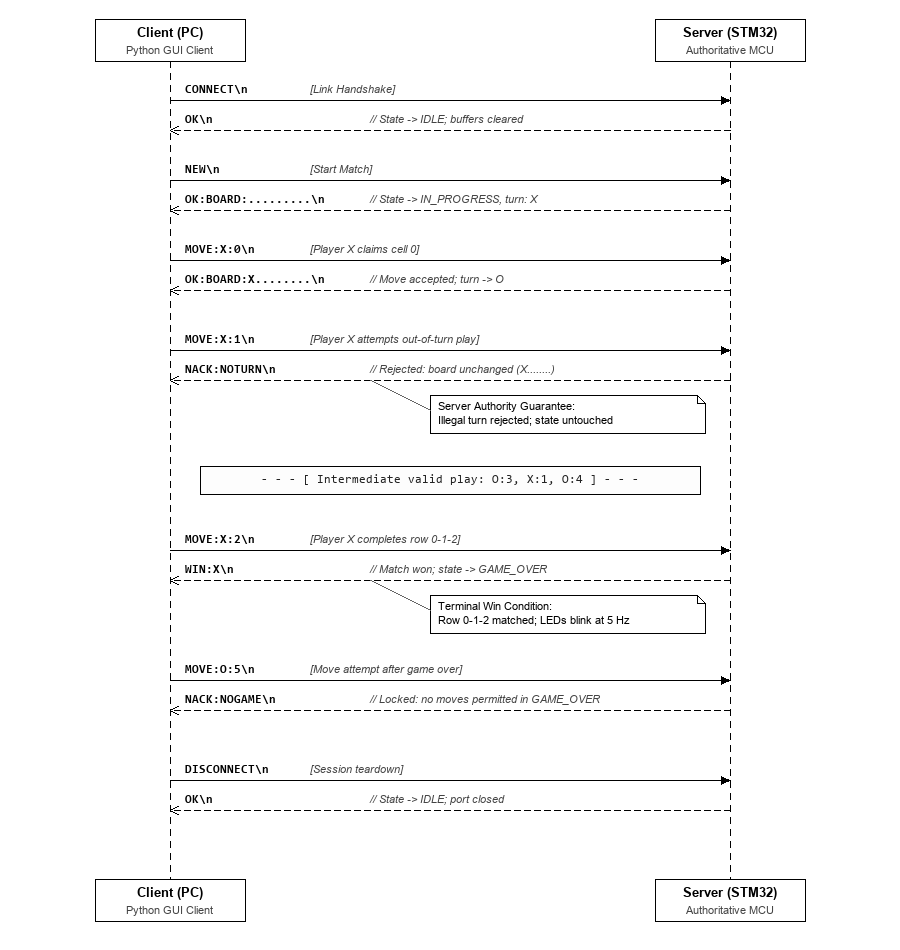
\includegraphics[width=\columnwidth]{figures/sequence_diagram.png}
\caption{Message sequence for a complete game: connect, two moves (the second
is rejected because it is out of turn), a scripted win sequence, and
disconnect. A rejected move leaves the board unchanged.}
\label{fig:sequence}
\end{figure}
